\section{Formale Definition}
\label{sec:model-definition}

Weil sie fähig sind, zeitliche Zustände zu speichern, eignen sich Rekurrente Neuronale Netze (in der restlichen Arbeit wird die Abkürzung «RNN» verwendet) besonders gut, um Sequenzen zu lernen.
Die natürliche Sprache ist eine Sequenz von Wörtern, die in sich wiederum aus einer Sequenz von Buchstaben bestehen.
Deshalb kommen RNNs bis heute in vielen Gebieten von natürlichsprachlicher Textverarbeitung zum Einsatz.

Die Besonderheit eines RNN's liegt darin, dass – anders als bei einfachen neuronalen Netzen – die \glspl{neuron} nicht nur den Wert der vorangehenden Netzschicht als
Eingangswert erhalten, sondern auch den Ausgangswert des vorangehenden Zeitschritts ihrer selbst.
Jedes \gls{neuron} speichert den Zustand der bisherigen Zeitschritte als sog. «hidden state», der mit der Variable $ h $ gekennzeichnet wird (siehe Abb. \ref{fig:rnn-model-definition}).
Für nähere Details zur Architektur und Funktionsweise sei auf die exzellente Beschreibung in \autocite{geron} verwiesen.

\begin{figure}
    \centering
    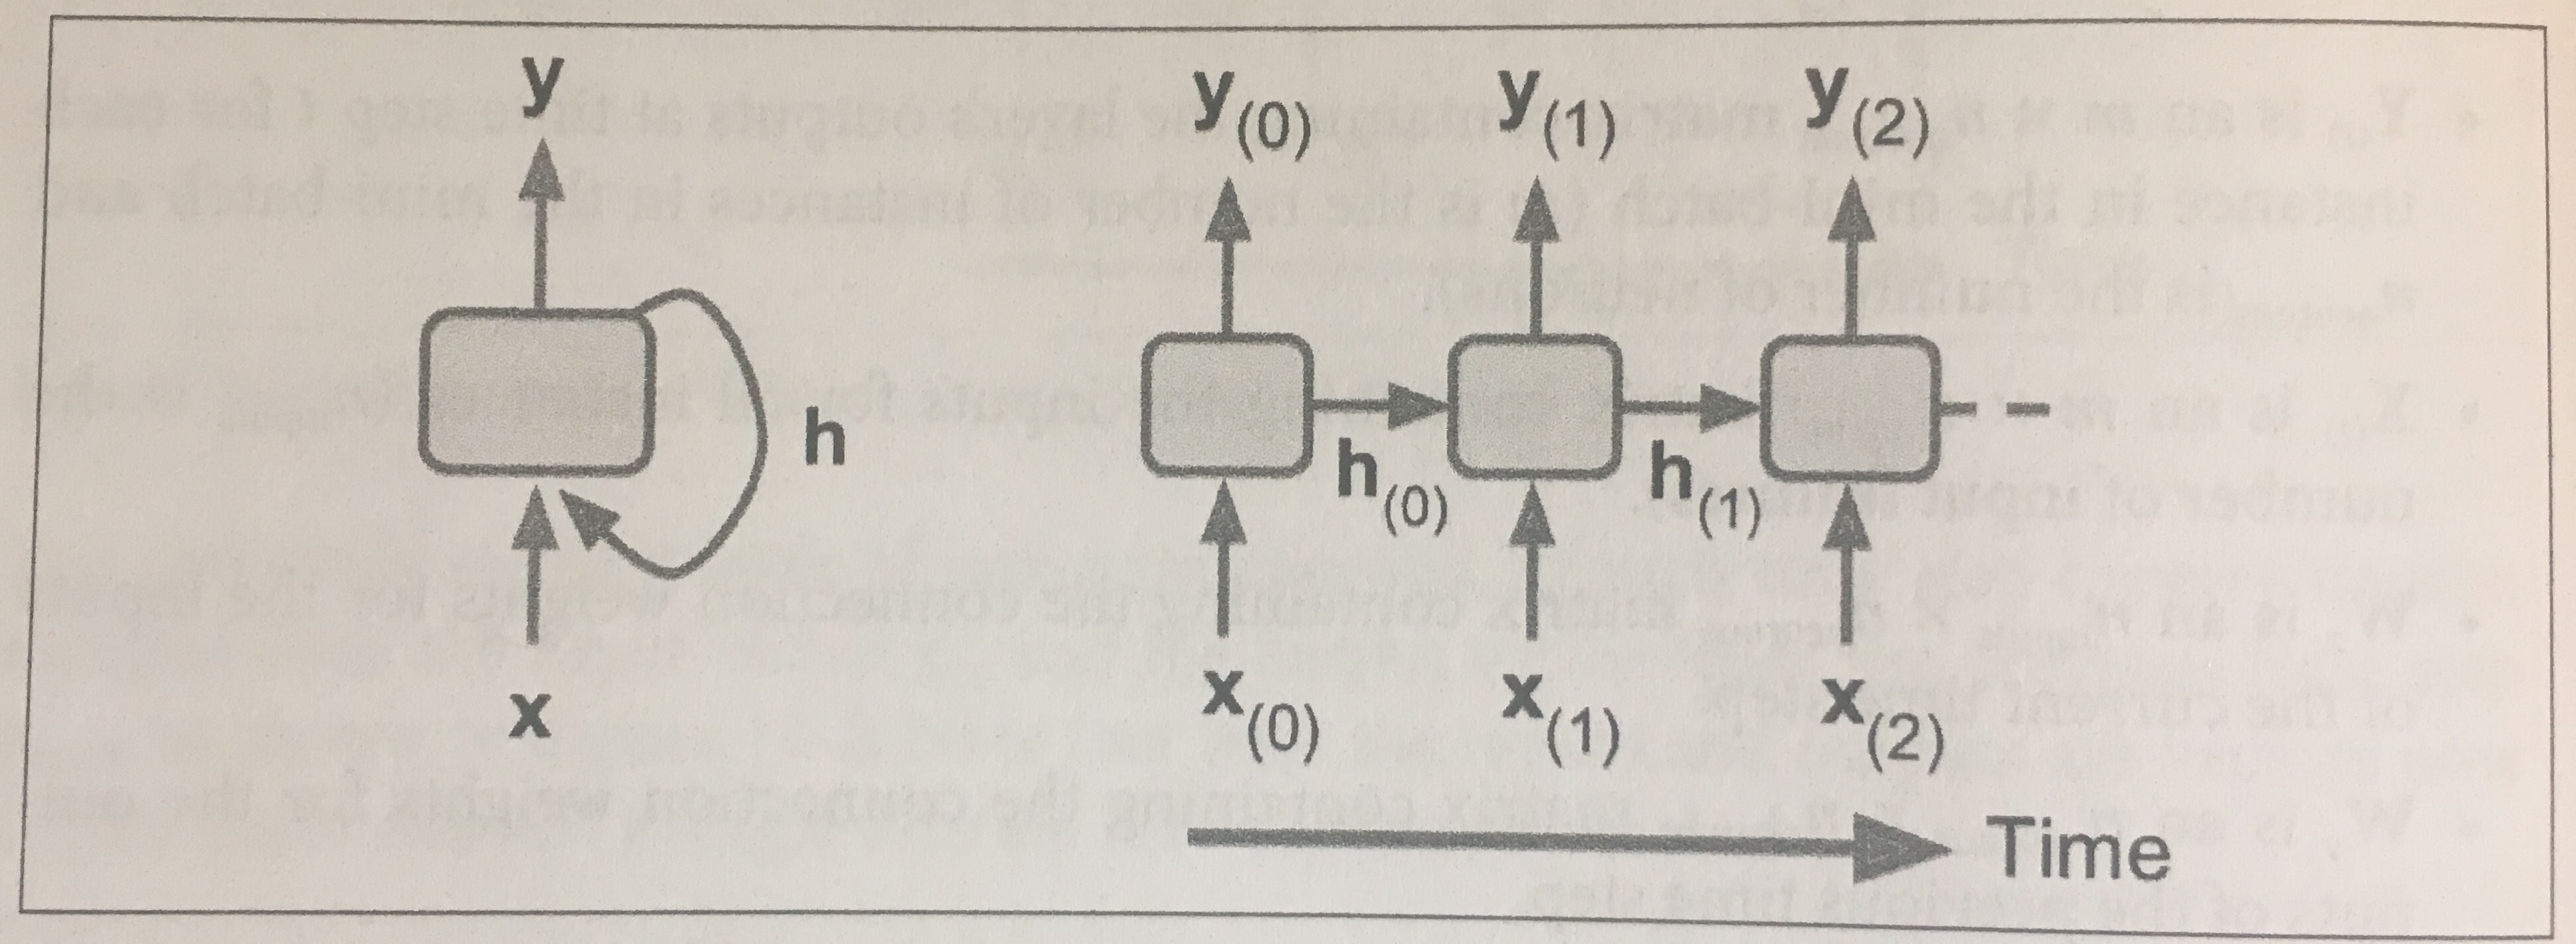
\includegraphics[width=0.75\linewidth]{images/model/model-rnn-definition.jpg}
    \caption[RNN Modell]{RNN Modell \autocite{geron}}
    \label{fig:rnn-model-definition}
\end{figure}

Zwei gut bekannte Probleme, die einfache RNN-Memory-Zellen aufweisen sind einerseits das sog. «Exploding/Vanishing Gradient Problem», bei dem insbesondere in mehrschichtigen neuronalen Netzen
die propagierten Werte «explodieren» oder gegen null «verschwinden», andererseits das Problem, dass anfangs eingespeiste Informationen gegen Ende der Sequenz verloren gehen \autocite{geron}.
Zur Lösung dieser Problem wurden sog. «Long-Short-Term Memory Cells» (LSTM)\autocite{lstm} und später sog. «Gated Recurrent Units» (GRU)\autocite{gru} entwickelt.
Weil sich beide «Gedächtniszellen» als sehr erfolgreich bewiesen haben, werden einfache RNN-Zellen schon fast nicht mehr verwendet.

